%!TEX root = ../Thesis.tex
\chapter{Analysis}\label{cha:analysis}
This chapter contains the analysis performed on the cases specified in section \ref{sec:cases}. 





    
    

% \section{Unsupervised dimensionallity reduction}\label{sec:dim_reduc}

%     \subsection{PCA}\label{subsec:PCA}


%     \subsection{Kernel PCA}\label{subsec:K_PCA}
    


% \section{Pelton needles}\label{sub:pelton_needles}
%     As mentioned, there was data available from three different power plants with pelton turbines. One of plants had recorded several issues with the needle control, and was used as a case to test early detection of problems with the needle operation. 
    
    
%     \begin{figure}
%         \centering
%         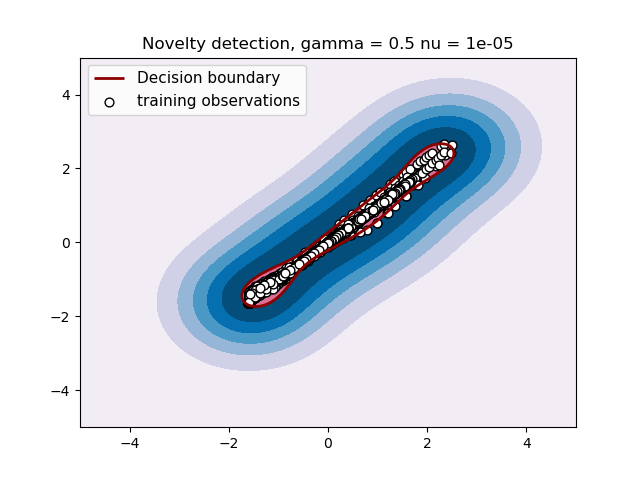
\includegraphics[scale=0.8]{report/figures/analysis/hjartdola/hjar_n2_4_novelty_05_1e-5_train.png}
%         \caption{OCSVM trained on data after overhaul in Mars 2017}
%         \label{fig:my_label}
%     \end{figure}


    
%     \begin{figure}
%         \centering
%         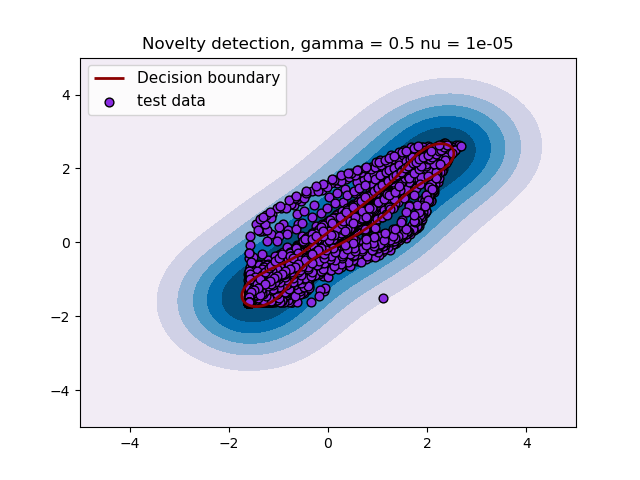
\includegraphics[scale=0.8]{report/figures/analysis/hjartdola/hjar_n2_4_novelty_05_1e-5_test.png}
%         \caption{All process data from before the overhaul}
%         \label{fig:my_label}
%     \end{figure}



